\documentclass[11pt]{report}

\usepackage[a4paper,margin=2.7cm]{geometry}
\usepackage{graphicx}
\usepackage{booktabs}
\usepackage{amsmath}
\usepackage{hyperref}
\usepackage{xcolor}
\usepackage{caption}
\usepackage{parskip}
\usepackage{fancyhdr}
\usepackage{titlesec}
\usepackage{seqsplit}

\hypersetup{colorlinks=true, linkcolor=blue!50!black, urlcolor=blue!50!black, citecolor=blue!50!black}
\captionsetup{font=small, labelfont=bf}
\titleformat{\chapter}[hang]{\normalfont\huge\bfseries}{\thechapter.}{1em}{}
\pagestyle{fancy}
\fancyhf{}
\fancyhead[L]{IMDC 2026 -- Data \& EDA Findings Report}
\fancyhead[R]{\thepage}
\renewcommand{\headrulewidth}{0.4pt}

\title{\textbf{Infodengue--Mosqlimate Dengue Challenge (IMDC) 2026\\[4pt]
\Large Data Audit and Exploratory Data Analysis: Findings Report}}
\author{Mosqlimate IMDC 2026 Project}
\date{\today}

\begin{document}

\maketitle
\thispagestyle{empty}

\begin{abstract}
\noindent
This report documents the data audit and exploratory data analysis (EDA) conducted on the official dataset of the 3rd Infodengue--Mosqlimate Dengue Challenge (IMDC 2026), an international sprint to forecast dengue (and chikungunya) case counts across Brazilian states. We describe the dataset's structure and provenance, verify its integrity and identify a data-leakage trap in the official backtesting design, and characterize the temporal, spatial, and covariate structure of the epidemiological signal. Headline findings: the dataset is structurally clean (100\% grid completeness, no duplicate or negative case records) but contains an unflagged 15-week gap between each backtest's training cutoff and evaluation window that must be filtered explicitly; the 2024 dengue season was an outlier of roughly four times the case volume of any other year in the 2011--2025 record; case incidence is strongly climate-lagged (temperature leading cases by approximately 12 weeks) and strongly stratified by Koppen climate class; and several auxiliary signals (chikungunya co-occurrence, Afya Whitebook search-access counts, Koppen/biome class) show exploitable structure for feature engineering. These findings motivate the modeling approach described in the concluding chapter and set up the next phase of the project: a leakage-safe backtesting harness and a comparison of statistical, machine-learning, deep-learning, and mechanistic forecasting models.
\end{abstract}

\tableofcontents

% ============================================================
\chapter{Background and Context}
% ============================================================

\section{The IMDC challenge}
The Infodengue--Mosqlimate Dengue Challenge (IMDC) is an international modeling sprint organized by the Mosqlimate project, in partnership with the InfoDengue surveillance platform, both based in Brazil (Getulio Vargas Foundation / Fiocruz-affiliated). The challenge asks research teams to produce probabilistic weekly forecasts of dengue -- and, optionally, chikungunya -- case counts across Brazilian states and cities, evaluated against both retrospective backtests and a genuine future season. The 3rd edition (2026) follows two prior editions (2024, 2025); the inaugural edition's ensemble-forecasting results were published in \emph{PNAS} (Araujo et al., 2026), which is the direct precedent for the journal paper this project is building toward.

\section{Project goal}
The present project participates in the 3rd IMDC as a registered team, with two linked deliverables: (i) a competitive submission following the challenge's official format and evaluation protocol, and (ii) a journal paper reporting the modeling methodology and results, in the spirit of the 1st edition's PNAS publication. This report covers the first phase of that work -- understanding the data well enough to build the forecasting pipeline on solid ground.

\section{Challenge structure, in brief}
The mandatory task is a weekly, state-level dengue forecast for 26 of Brazil's 27 states (Espirito Santo is excluded). Three optional tracks add city-level dengue (15 cities) and state- and city-level chikungunya (10 cities). Each track requires two kinds of submission: a \emph{validation} phase, consisting of four retrospective backtests against known past seasons, and a \emph{forecast} phase, predicting the true upcoming 2026--2027 season. Forecasts must be probabilistic: a median plus 50\%, 80\%, 90\%, and 95\% prediction intervals for every week of the target season.

% ============================================================
\chapter{The Dataset}
% ============================================================

\section{Provenance and access}
The official IMDC 2026 dataset (\texttt{data\_imdc\_2026}) is distributed by Mosqlimate via an FTP server (\texttt{info.dengue.mat.br}) and mirrors data also available through the Mosqlimate API. It bundles epidemiological, climate, oceanic, demographic, and behavioral-proxy data for all 5{,}570 Brazilian municipalities. The full archive is approximately 800\,MB compressed.

\section{Contents}
Table~\ref{tab:datasets} summarizes the twelve files in the archive.

\begin{table}[htbp]
\centering
\small
\begin{tabular}{@{}p{3.0cm}p{6.1cm}p{2.1cm}p{2.1cm}@{}}
\toprule
\textbf{File} & \textbf{Content} & \textbf{Resolution} & \textbf{Coverage} \\
\midrule
\seqsplit{dengue.csv.gz} & Weekly dengue case counts, SINAN/IBGE via InfoDengue & Weekly, municipality & 2010-01 -- 2026-03 \\
\seqsplit{chikungunya.csv.gz} & Weekly chikungunya case counts & Weekly, municipality & 2013-12 -- 2026-03 \\
\seqsplit{climate.csv.gz} & ERA5 reanalysis: temperature, precipitation, pressure, humidity & Weekly, municipality & 1999-12 -- 2026-03 \\
\seqsplit{forecasting\_climate.csv.gz} & ECMWF System 51 seasonal climate forecast, up to 6 months ahead & Monthly, municipality & 2010-01 -- 2026-03 \\
\seqsplit{ocean\_climate\_oscillations.csv.gz} & ENSO, IOD, PDO indices & Weekly, national & 1993 -- 2026 \\
\seqsplit{environ\_vars.csv.gz} & Koppen climate class, biome & Static, municipality & -- \\
\seqsplit{datasus\_population\_2001\_2025.csv.gz} & Population estimates & Yearly, municipality & 2001 -- 2025 \\
\seqsplit{access\_afya\_dengue\_2021\_2026.csv.gz} & Afya Whitebook dengue-related search-access counts & Daily, municipality & 2021 -- 2026 \\
\seqsplit{map\_regional\_health.csv} & Municipality $\to$ health-region/state hierarchy & Static & -- \\
\seqsplit{shape\_*.gpkg} (3 files) & Municipality / regional / macroregional health geometries & Static & -- \\
\bottomrule
\end{tabular}
\caption{Files in the official IMDC 2026 dataset.}
\label{tab:datasets}
\end{table}

\section{Case-data schema and the backtest fold design}
The two case-count tables (\texttt{dengue.csv.gz}, \texttt{chikungunya.csv.gz}) carry, alongside \texttt{geocode}, \texttt{date}, \texttt{casos}, \texttt{uf} and health-region codes, eight boolean columns \texttt{train\_1..train\_4} / \texttt{target\_1..target\_4} that mark, for each of the four official backtests, which rows belong to the training window and which belong to the evaluation window. A \texttt{target\_city} flag marks the 15 (dengue) / 10 (chikungunya) municipalities used for the optional city-level tracks.

We derived the four fold boundaries directly from these flags rather than trusting written documentation (Table~\ref{tab:folds}). Each backtest's training window always starts on 2010-01-03; the four folds' cutoffs step forward by exactly one year, terminating around mid-June of years 2022--2025, with each evaluation window running from early October of that year through late September/early October of the following year -- the Brazilian dengue season.

\begin{table}[htbp]
\centering
\begin{tabular}{@{}lccc@{}}
\toprule
\textbf{Fold} & \textbf{Train cutoff} & \textbf{Target window} & \textbf{Gap (weeks)} \\
\midrule
1 & 2022-06-19 & 2022-10-09 -- 2023-10-01 & 15 \\
2 & 2023-06-18 & 2023-10-08 -- 2024-09-29 & 15 \\
3 & 2024-06-16 & 2024-10-06 -- 2025-09-28 & 15 \\
4 & 2025-06-15 & 2025-10-05 -- 2026-03-08 & 15 \\
\bottomrule
\end{tabular}
\caption{Official backtest fold boundaries, derived from the \texttt{train\_N}/\texttt{target\_N} flags in \texttt{dengue.csv.gz} (identical for chikungunya).}
\label{tab:folds}
\end{table}

\subsection*{A confirmed data-leakage trap}
Between every fold's training cutoff and the start of its target window there is a gap of exactly \textbf{15 weeks} that is flagged \texttt{False} for both \texttt{train\_N} and \texttt{target\_N} (e.g., fold 1: 2022-06-26 through 2022-10-02). These rows contain real, unmasked case counts. A training-data filter written as ``\texttt{NOT target\_N}'' -- a natural first instinct -- will silently include these 15 weeks of future-relative-to-cutoff data in the training set. We confirmed this experimentally and built an explicit-cutoff filter (\texttt{date} $\leq$ \texttt{train\_cutoff}) instead, verified by an automated regression test that reproduces the leak under the naive filter and confirms its absence under the explicit one. This applies to \emph{every} joined table: the auxiliary tables (climate, ocean indices, access data) carry no fold flags at all, so the same explicit-cutoff discipline must be reapplied by hand at every feature join.

\subsection*{Fold 4 is only partially resolved}
Fold 4's evaluation window nominally covers the 2025--2026 season (2025-10-05 through late September 2026), but the dataset's case records currently end at 2026-03-08 -- the same date across every table, consistent with normal surveillance reporting lag rather than a data error. In practice, fold 4 can only be scored against roughly the first five months of its target season until the data is refreshed closer to the real forecast deadline.

\section{Structural integrity}
Table~\ref{tab:integrity} summarizes the structural checks run against every table. The dataset is very clean: perfect municipality$\times$week grid completeness for the case, climate, and access tables; no duplicate \texttt{(geocode, date)} rows; no negative case counts; and every case-data date falls on a Sunday, matching the submission format's date requirement exactly.

\begin{table}[htbp]
\centering
\small
\begin{tabular}{@{}p{7.7cm}p{7cm}@{}}
\toprule
\textbf{Check} & \textbf{Result} \\
\midrule
Dengue: rows vs. expected municipality$\times$week grid & 4{,}706{,}650 / 4{,}706{,}650 (100.0\%) \\
Chikungunya: rows vs. expected grid & 3{,}548{,}090 / 3{,}548{,}090 (100.0\%) \\
Climate: rows vs. expected grid & 7{,}621{,}223 / 7{,}621{,}223 (100.0\%) \\
Access (Afya): rows vs. expected grid & 8{,}963{,}730 / 8{,}963{,}718 (100.0\%, 12 duplicate rows) \\
Duplicate \texttt{(geocode, date)} rows, dengue/chikungunya & 0 \\
Negative case counts & 0 \\
Non-Sunday dates & 0 \\
Missing UFs / states & 0 (all 27 present; Esp\'irito Santo excluded downstream) \\
Target-city lists (dengue 15 / chikungunya 10) & Match official specification exactly \\
\bottomrule
\end{tabular}
\caption{Structural integrity checks across the raw dataset.}
\label{tab:integrity}
\end{table}

A small number of minor anomalies were found and documented for downstream handling: three municipalities (geocodes 2916104, 2919926 in Bahia and 2605459 in Pernambuco) are entirely absent from \texttt{climate.csv.gz}; the same Pernambuco municipality accounts for all 1{,}080 missing values in \texttt{forecasting\_climate.csv.gz}; one population-table geocode (5101837, population 5{,}877 in 2025 only) does not appear in any other table, consistent with a newly split municipality with no case history; and the 12 duplicate rows in the access table carry differing \texttt{access\_count} values and must be summed rather than dropped. None of these affect more than a handful of the 5{,}570 municipalities and none materially affects state-level aggregation.

% ============================================================
\chapter{Exploratory Data Analysis}
% ============================================================

All analysis in this chapter uses case counts aggregated from municipality to state level (summed within each of the 26 mandatory states), since that is the unit the challenge actually scores.

\section{National trends: an unprecedented 2024 epidemic}

\begin{figure}[htbp]
\centering
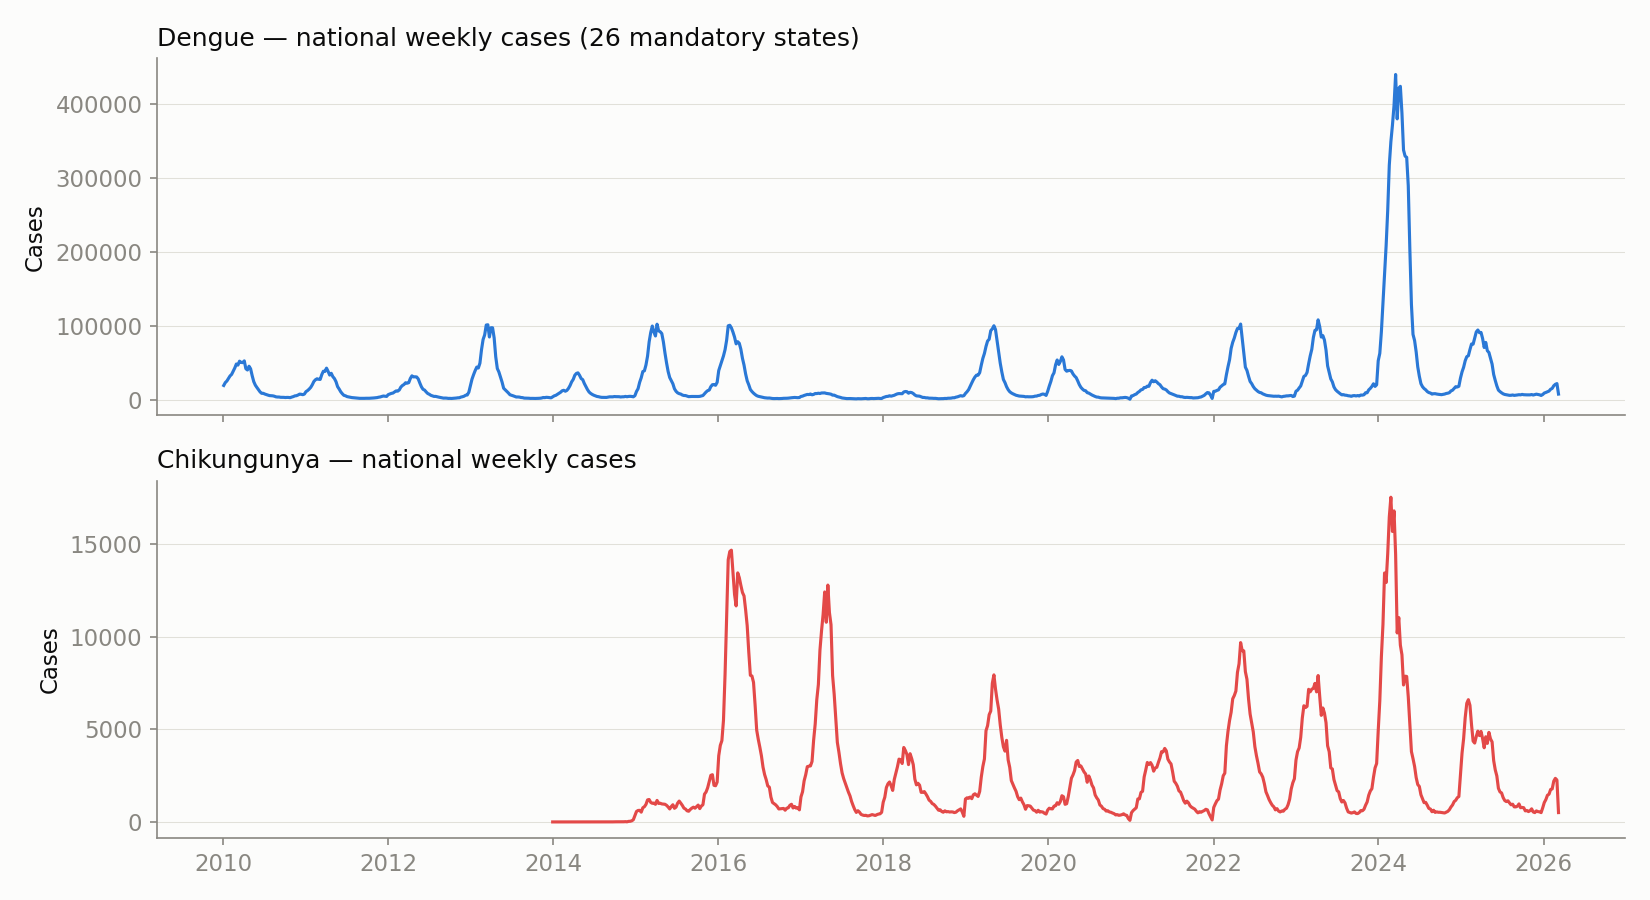
\includegraphics[width=0.95\textwidth]{../results/figures/national_weekly_trends.png}
\caption{National weekly case counts, dengue (top) and chikungunya (bottom), 2010--2026, summed across the 26 mandatory states.}
\label{fig:national_trends}
\end{figure}

Figure~\ref{fig:national_trends} shows fifteen years of dengue seasonality with a clearly anomalous 2024 season: a peak of 440{,}538 national weekly cases (week of 2024-03-17), against a typical seasonal peak of 40{,}000--100{,}000 cases in every other year in the record. The 2024 annual total, 6.67 million cases, is roughly four times the next-largest year (2023, 1.64 million) and roughly nine times the 2011--2025 median annual total (1.38 million). Chikungunya shows a similar, though smaller, elevated 2024 season (peak 17{,}521 weekly cases) atop a roughly biennial epidemic pattern (visible peaks in 2016, 2017/19, 2022/23, 2024) consistent with the disease's slower buildup of population susceptibility between outbreaks.

\textbf{Interpretation.} The 2024 season is a genuine outlier, not a data artifact -- it is corroborated in both diseases and is consistent with Brazil's widely reported record-breaking 2024 dengue epidemic. For modeling, this has two consequences: (i) any model trained naively on raw scale will be dominated by 2024 and under-fit typical seasons, arguing for log/log1p-scale modeling and loss functions, and (ii) 2024 falls inside backtest fold 2's target window (2023-10-08 -- 2024-09-29) and fold 3's training window, so both the difficulty of scoring fold 2 and the risk of the outlier year distorting fold-3-onward training deserve explicit attention during model evaluation.

\section{Seasonality}

\begin{figure}[htbp]
\centering
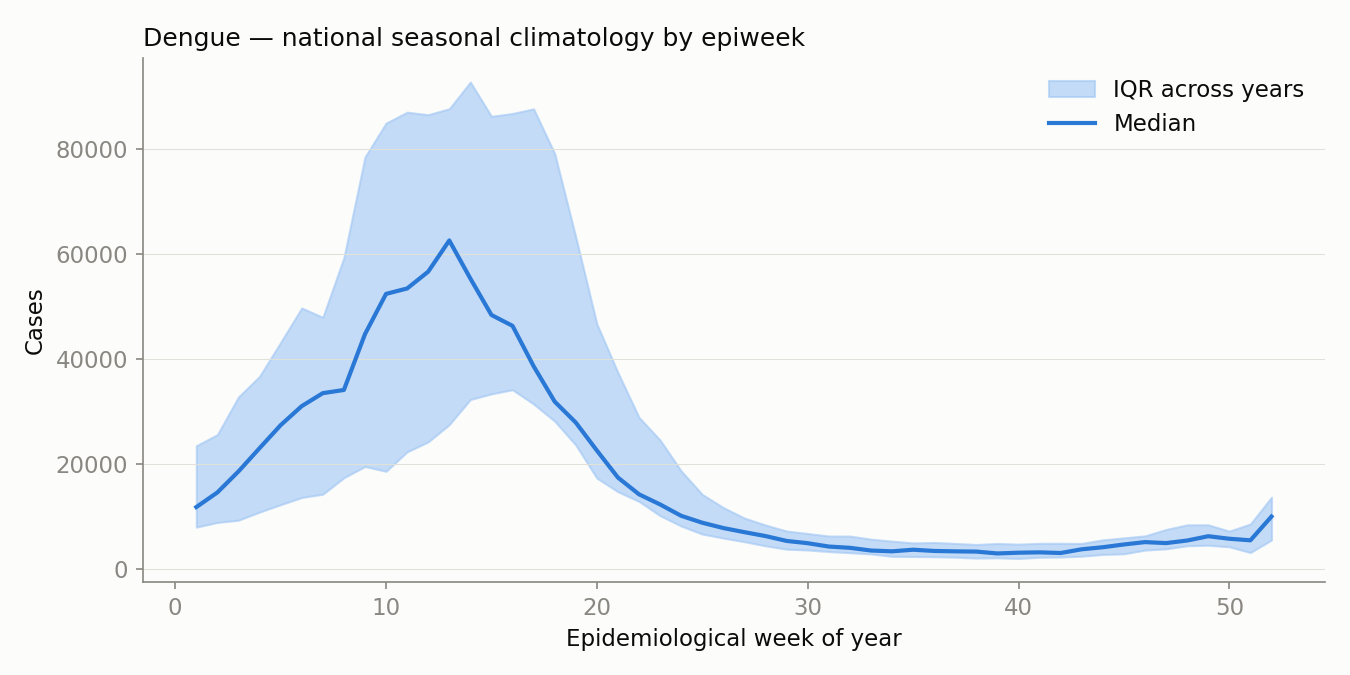
\includegraphics[width=0.85\textwidth]{../results/figures/dengue_climatology.png}
\caption{National dengue seasonal climatology: median weekly case count and interquartile range across all observed years, by epidemiological week of year.}
\label{fig:climatology}
\end{figure}

\begin{figure}[htbp]
\centering
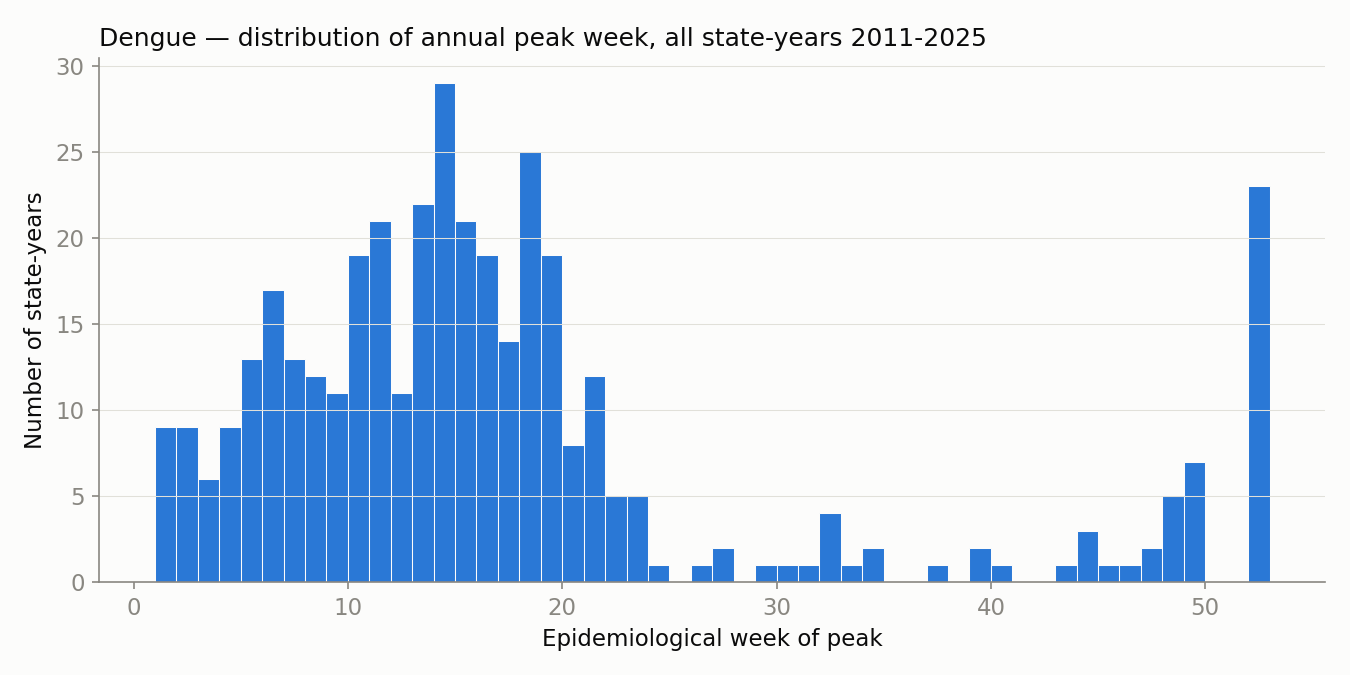
\includegraphics[width=0.75\textwidth]{../results/figures/dengue_peak_week_distribution.png}
\caption{Distribution of the epidemiological week of the annual peak, across all state-years, 2011--2025.}
\label{fig:peak_week}
\end{figure}

Figure~\ref{fig:climatology} confirms a single, strong annual peak nationally, centered in the first third of the year, consistent with the Southern Hemisphere's summer/rainy season. Figure~\ref{fig:peak_week} shows this national pattern masks meaningful state-level spread: the median state-year peak falls at epidemiological week 14, but the interquartile range spans weeks 9--19 -- a ten-week window.

\textbf{Interpretation.} A single national seasonal prior is a reasonable starting point but will systematically mistime the peak for many individual states. Per-state or per-region seasonal offsets (e.g., a state- or macroregion-level harmonic feature, or state random effects in a hierarchical model) are likely to materially improve peak-timing accuracy, one of the metrics this project intends to report alongside probabilistic scores.

\section{Spatial heterogeneity}

\begin{figure}[htbp]
\centering
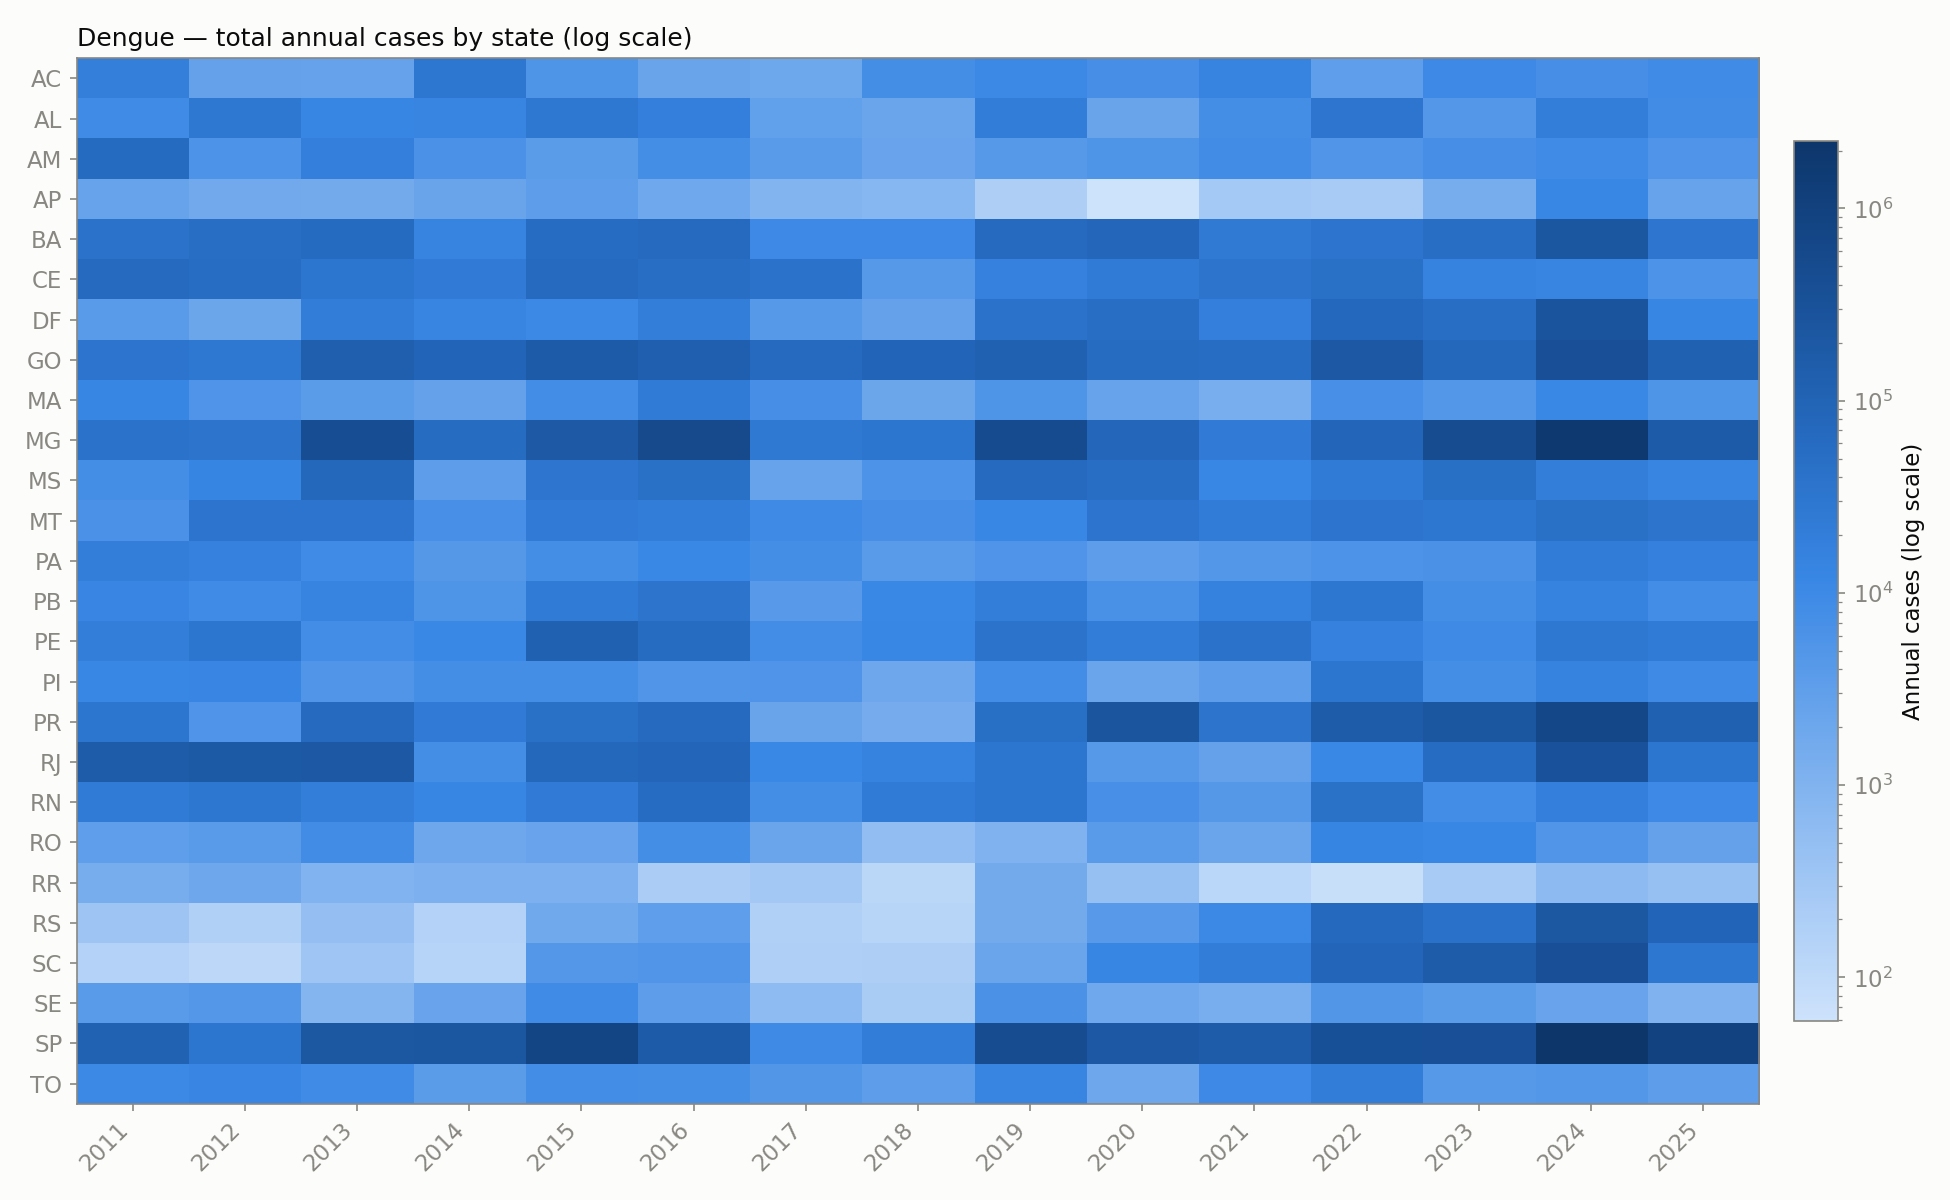
\includegraphics[width=0.95\textwidth]{../results/figures/dengue_state_year_heatmap.png}
\caption{Total annual dengue cases by state and year, 2011--2025, log scale.}
\label{fig:heatmap}
\end{figure}

\begin{figure}[htbp]
\centering
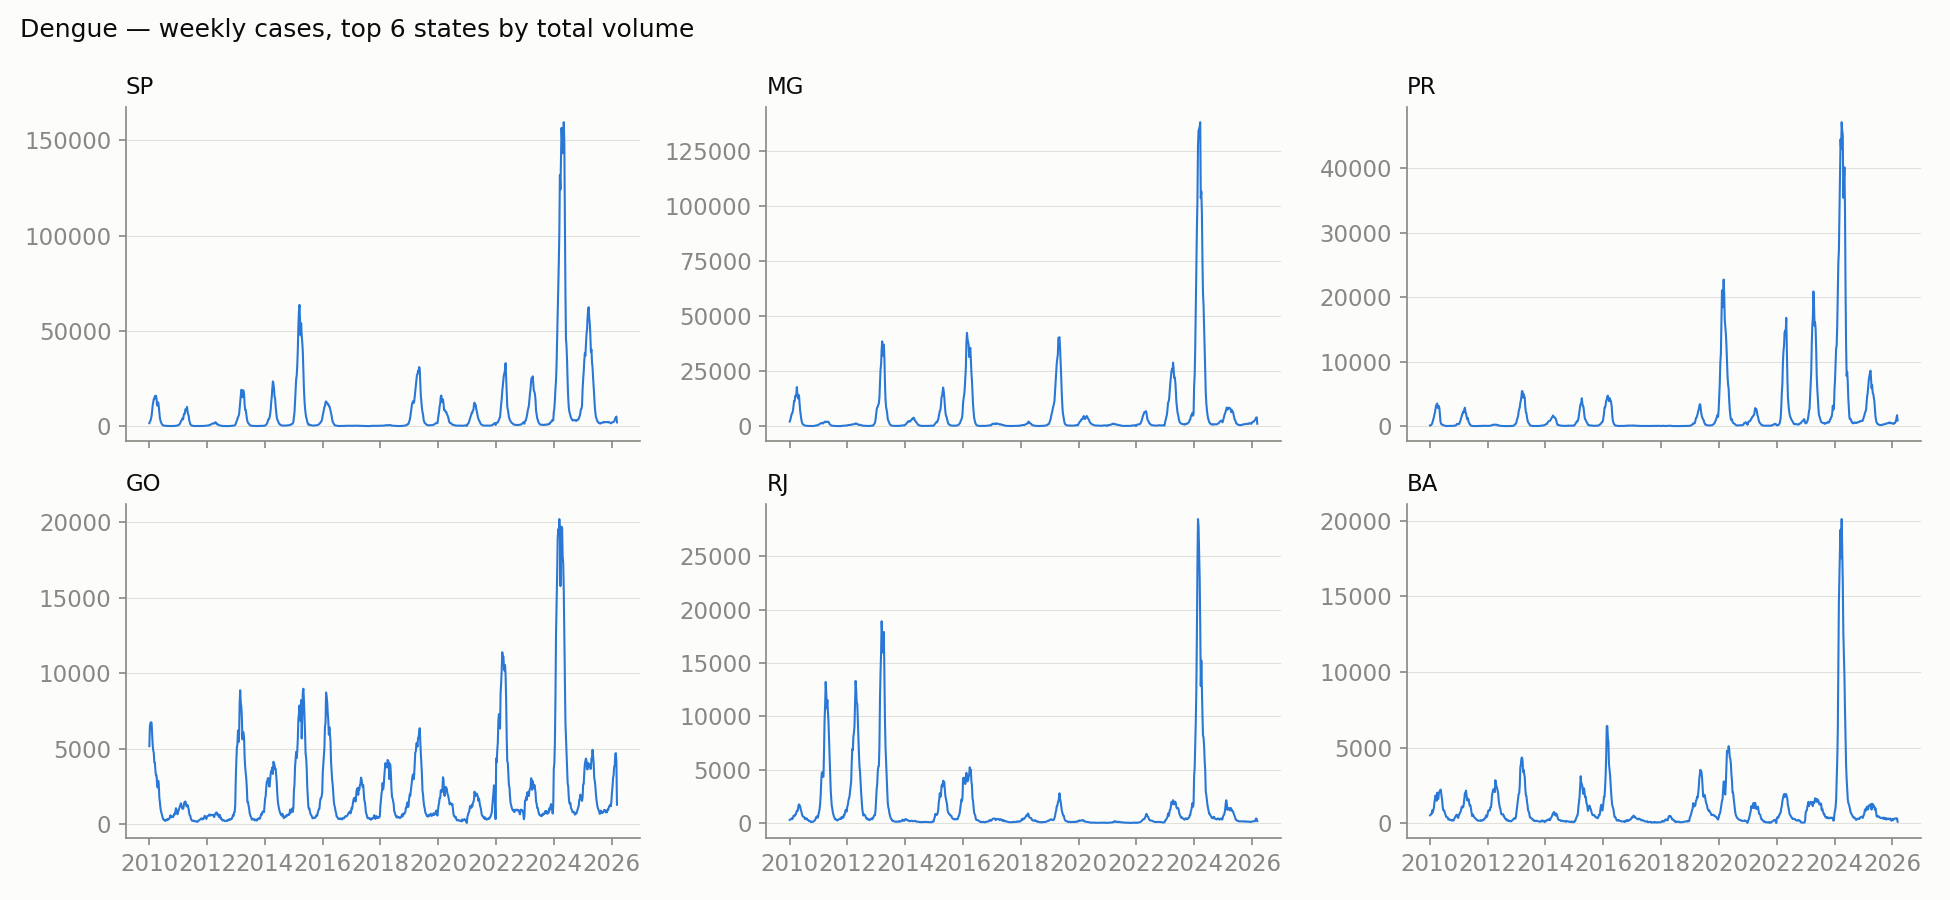
\includegraphics[width=0.95\textwidth]{../results/figures/dengue_top6_states_small_multiples.png}
\caption{Weekly dengue case counts for the six states with the largest cumulative case volume, 2010--2026.}
\label{fig:top6}
\end{figure}

By cumulative 2011--2025 case volume, the six largest states are S\~ao Paulo (6.24M), Minas Gerais (4.34M), Paran\'a (1.74M), Goi\'as (1.73M), Rio de Janeiro (1.21M), and Bahia (0.84M) -- together accounting for a large majority of the national burden (Figures~\ref{fig:heatmap}--\ref{fig:top6}). More striking than the ranking itself is a visible trend in Figure~\ref{fig:heatmap}: the traditionally low-incidence southern states (Rio Grande do Sul, Santa Catarina) show a clear darkening -- rising incidence -- in the more recent years of the record, consistent with the well-documented southward range expansion of \emph{Aedes aegypti} transmission in Brazil under a warming climate.

\textbf{Interpretation.} Case volume is extremely right-skewed across states (several orders of magnitude between the largest and smallest), which reinforces the case for log-scale modeling and for scale-free evaluation (e.g., relative WIS against a baseline) rather than raw-scale error metrics that would be dominated by S\~ao Paulo and Minas Gerais. The apparent southward-expansion trend is worth testing formally (e.g., a state-level time trend term) since it implies the historical climatology of southern states is becoming a weaker guide to their future risk -- directly relevant to how much weight a forecasting model should place on long historical baselines for those states specifically.

\section{Dengue and chikungunya co-occurrence}

\begin{figure}[htbp]
\centering
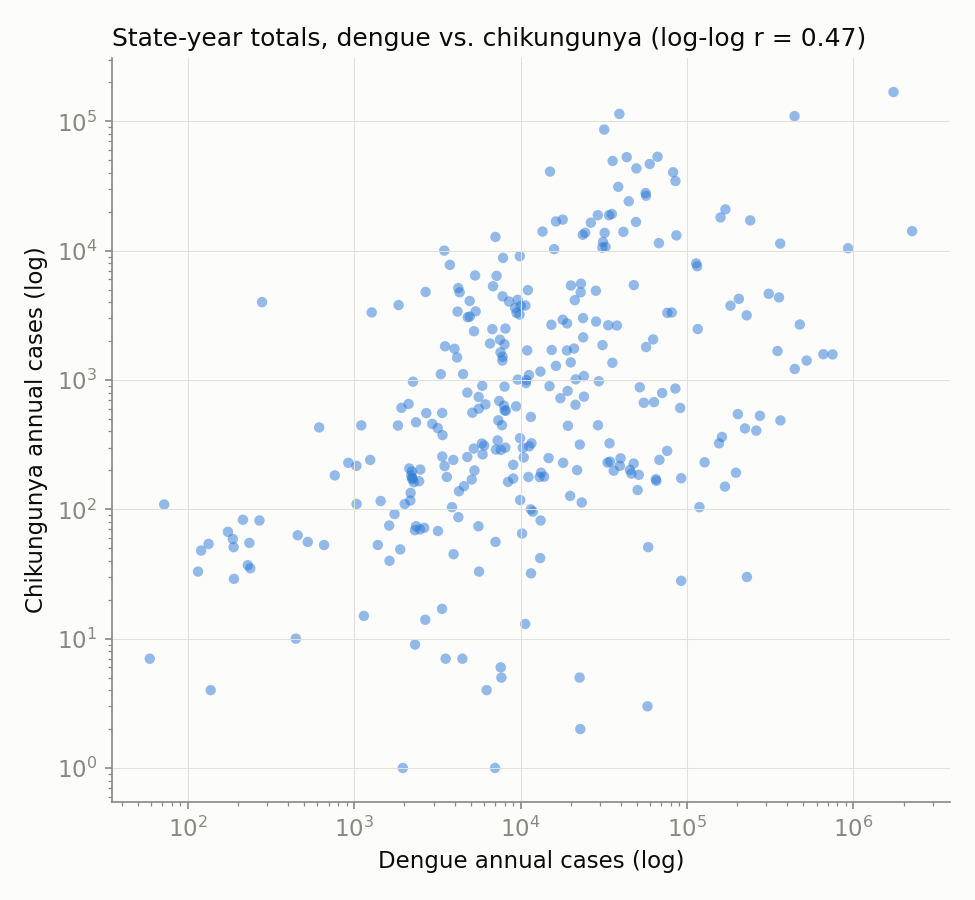
\includegraphics[width=0.65\textwidth]{../results/figures/dengue_vs_chik_state_year_scatter.png}
\caption{State-year total case counts, dengue vs.\ chikungunya (log-log axes).}
\label{fig:dengue_chik}
\end{figure}

Figure~\ref{fig:dengue_chik} shows a moderate positive association between the two diseases' annual state-level totals (log-log Pearson $r = 0.51$, $n=335$ state-years with non-zero counts in both diseases) -- expected, since both are transmitted by \emph{Aedes aegypti} and respond to overlapping climate drivers, but far from a 1:1 relationship.

\textbf{Interpretation.} The correlation is strong enough to be worth testing as an auxiliary signal (e.g., a multi-task or chikungunya-as-covariate model for dengue) but not strong enough that one disease can stand in for the other; both need to be modeled on their own case histories, consistent with the challenge's requirement to forecast them as separate tracks.

\section{Climate lead-lag structure}

\begin{figure}[htbp]
\centering
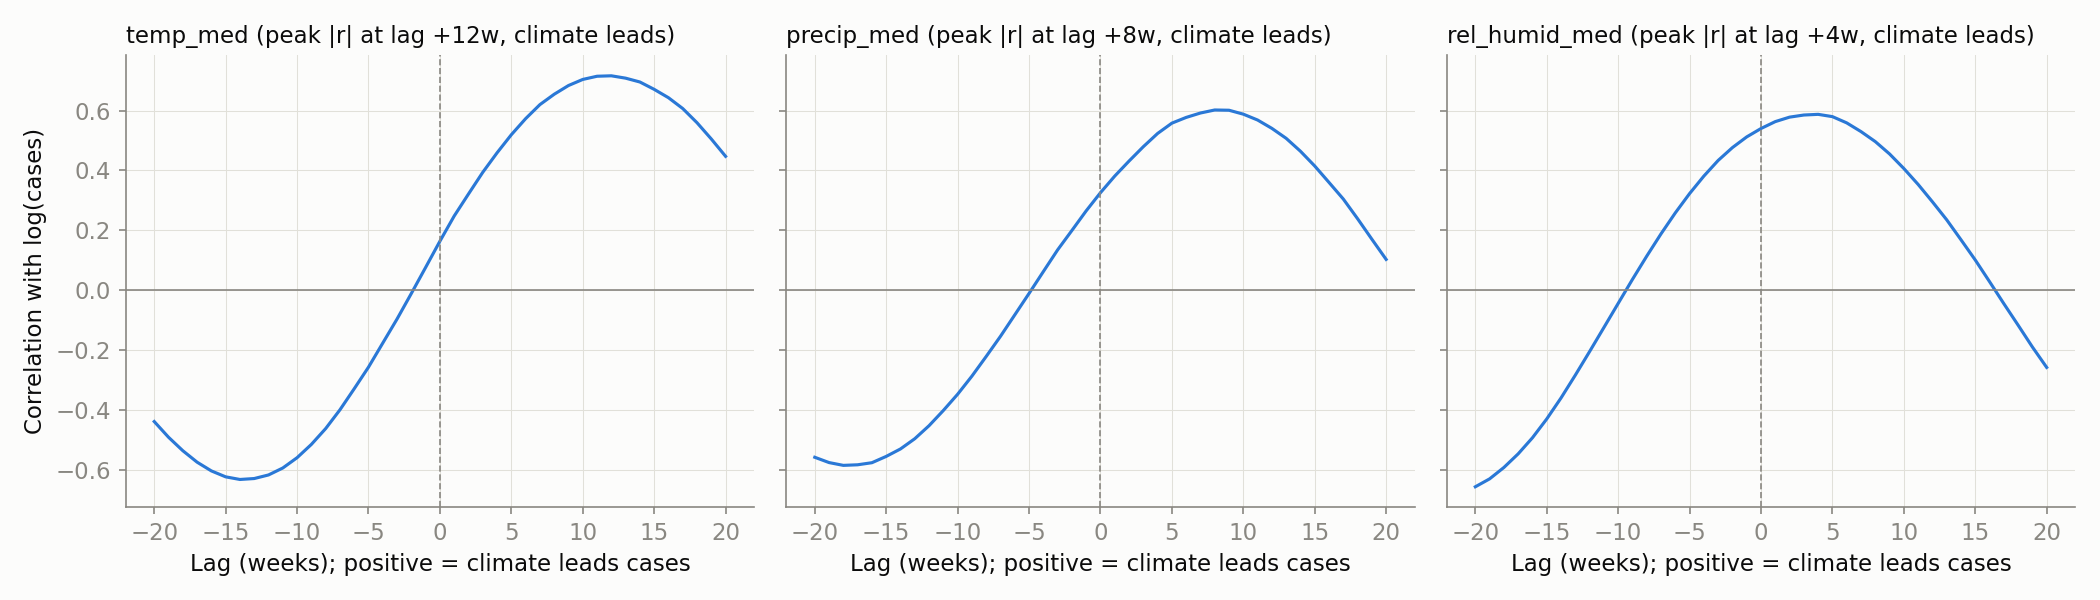
\includegraphics[width=\textwidth]{../results/figures/climate_lag_cross_correlation.png}
\caption{Cross-correlation of national log-case-counts against population-weighted national climate variables at lags of $-20$ to $+20$ weeks. Positive lag means the climate variable leads case counts.}
\label{fig:climate_lag}
\end{figure}

We cross-correlated log-transformed national weekly case counts against population-weighted national climate variables at lags from $-20$ to $+20$ weeks (Figure~\ref{fig:climate_lag}). All three variables show physically sensible positive-lag peaks: mean temperature leads cases by approximately 12 weeks ($r=0.72$), precipitation by approximately 8 weeks ($r=0.60$), and relative humidity by approximately 4 weeks ($r=0.59$). This ordering and magnitude is consistent with the known biological chain from favorable weather to mosquito breeding and population growth, through the extrinsic incubation period, to symptomatic, diagnosed, and reported cases.

We note an important methodological caveat, discovered and corrected during this analysis: because both case counts and climate variables carry strong annual (\textasciitilde52-week) seasonality, a naive cross-correlation over a wide lag window is partly confounded by that shared cycle and can produce a sinusoid-shaped correlation curve independent of any genuine short-term causal lag. The lags reported here should be treated as an informative prior for feature-window design, not a precise causal estimate; a deseasonalized (e.g.\ STL-residual) cross-correlation is planned as a follow-up before finalizing lag-feature windows for the modeling pipeline. (A related sign-convention bug in the analysis code -- an inverted lag-direction label -- was caught via a synthetic-data sanity check and corrected before being propagated into any feature-engineering decision.)

\section{Ocean oscillation indices}

\begin{figure}[htbp]
\centering
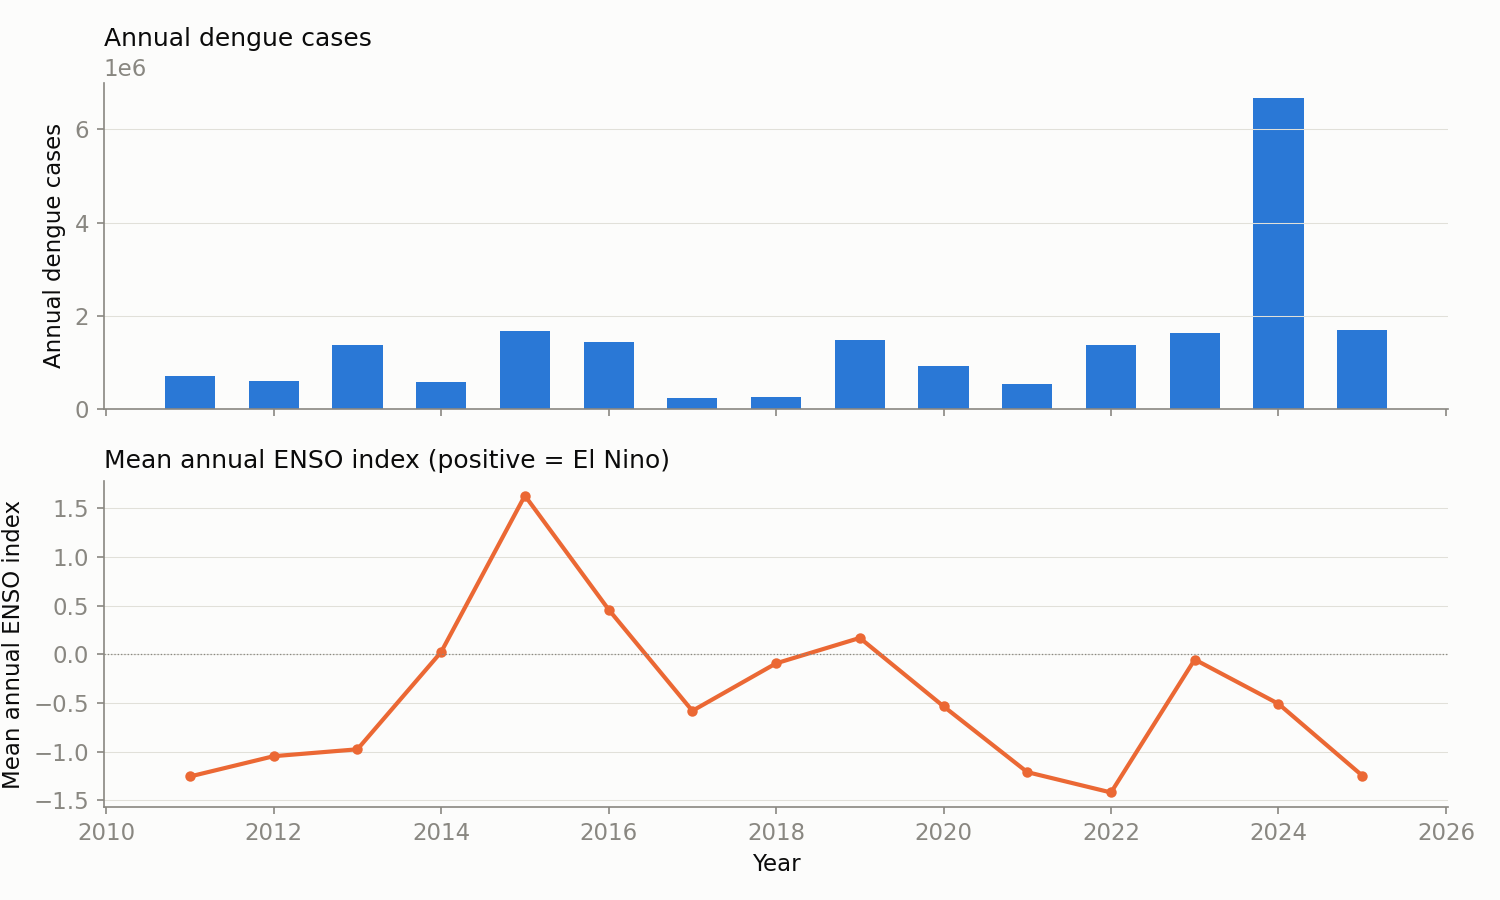
\includegraphics[width=0.85\textwidth]{../results/figures/dengue_vs_enso_annual.png}
\caption{Annual national dengue case totals and mean annual ENSO index, 2011--2025.}
\label{fig:enso}
\end{figure}

The correlation between annual national case totals and the mean annual ENSO (El Ni\~no--Southern Oscillation) index is weak ($r=0.07$; Figure~\ref{fig:enso}).

\textbf{Interpretation.} This near-null result at the national-annual level is not necessarily a null result for ENSO's relevance -- El Ni\~no's effect on Brazilian rainfall is known to be spatially heterogeneous (wetter in some regions, drier in others), so a single national scalar per year likely averages away a real, but regionally opposite-signed, signal. ENSO (and the other ocean indices, IOD and PDO) should be re-tested as region- or state-level features, and at weekly rather than annual resolution, before being ruled out.

\section{The Afya Whitebook search-access signal}

\begin{figure}[htbp]
\centering
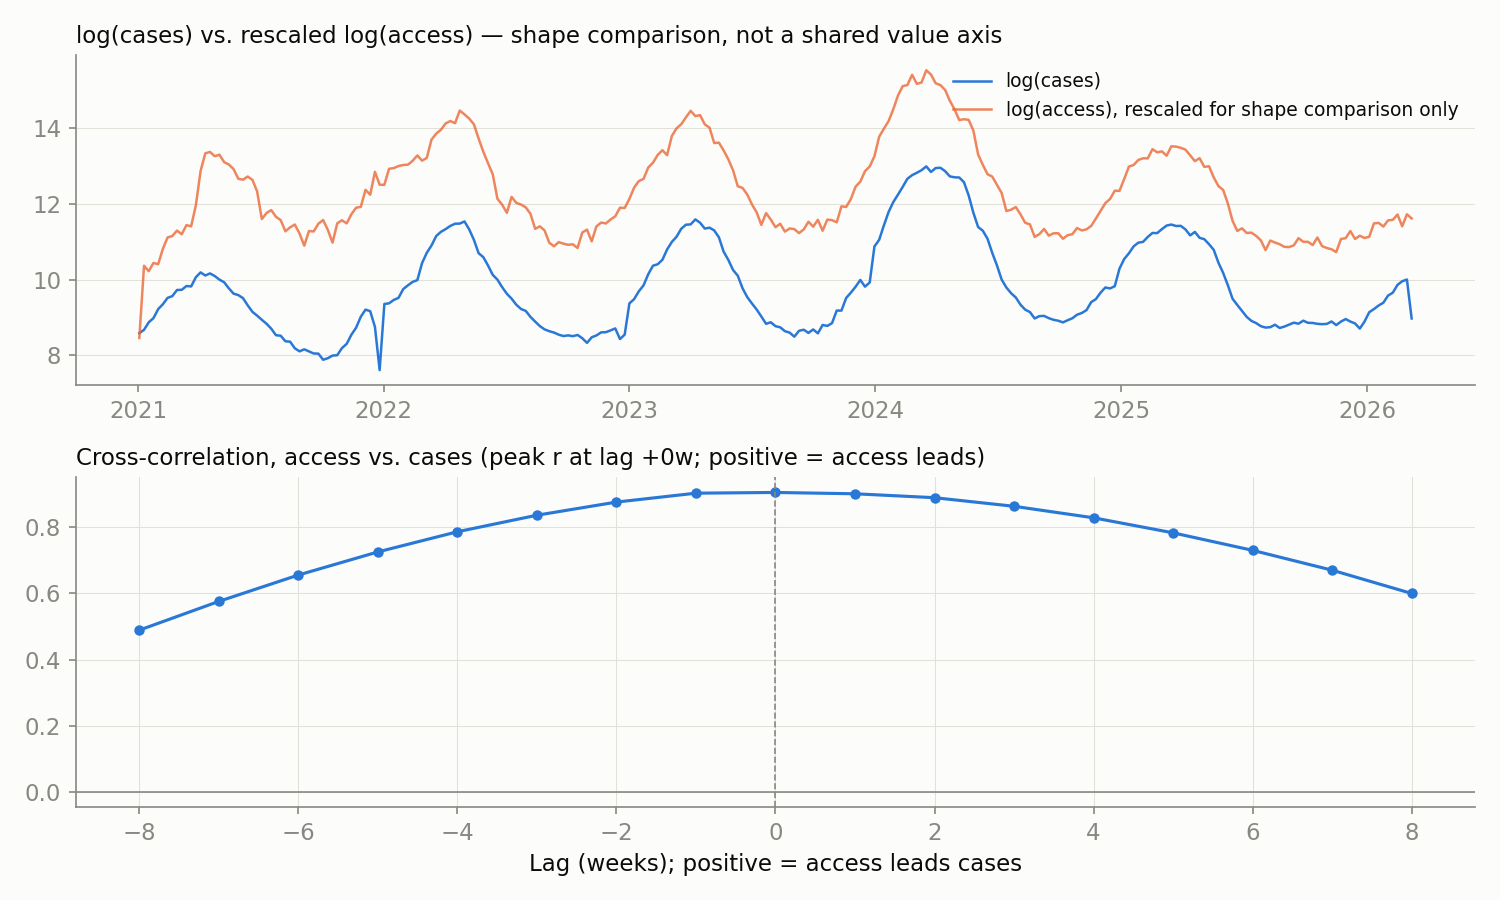
\includegraphics[width=0.85\textwidth]{../results/figures/access_afya_vs_cases.png}
\caption{Top: log-transformed national weekly case counts and rescaled log search-access counts (2021--2026). Bottom: cross-correlation at lags of $-8$ to $+8$ weeks.}
\label{fig:access}
\end{figure}

Search-access counts from the Afya Whitebook medical reference (available 2021 onward) track national case counts closely: the cross-correlation peaks at lag 0 with $r=0.90$, and is nearly symmetric, remaining at $r=0.90$ at lag $+1$ and $r=0.87$ at lag $-1$ (Figure~\ref{fig:access}).

\textbf{Interpretation.} At the national weekly resolution tested here, the access signal behaves as a strong \emph{contemporaneous} correlate of reported cases rather than a clearly leading indicator -- the peak sits at lag 0, not at a positive lag as a genuine early-warning signal would show. It remains a plausible nowcasting feature specifically for the most recent 1--2 weeks before a forecast origin, where official case counts are themselves incomplete due to reporting lag (the mechanism already identified as the likely cause of the dataset's own right-censoring, Section~2.3); its value there depends on whether search behavior is reported with less delay than case confirmation, which this national-level analysis cannot resolve on its own and should be tested directly at the point features are engineered.

\section{Climate class and biome}

\begin{figure}[htbp]
\centering
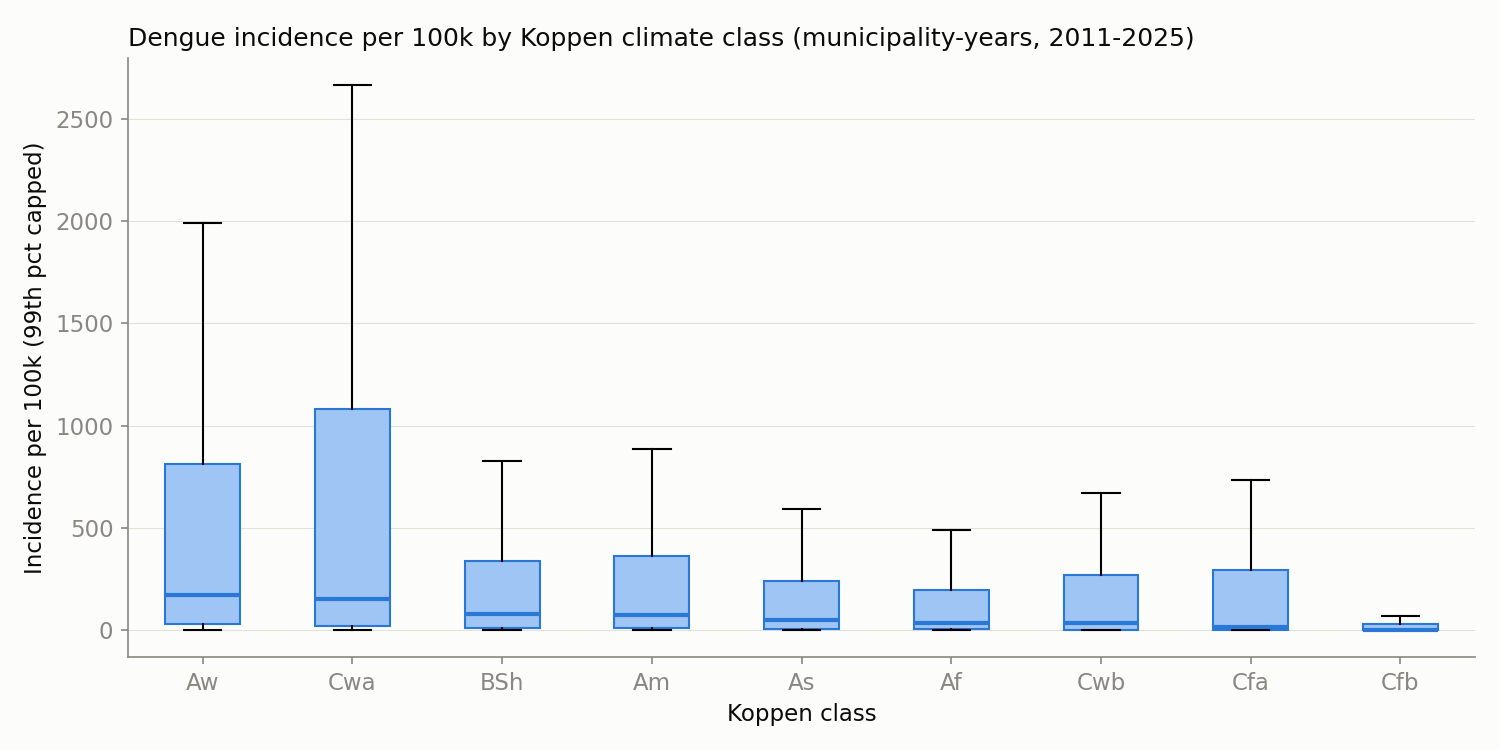
\includegraphics[width=0.85\textwidth]{../results/figures/dengue_incidence_by_koppen.png}
\caption{Distribution of municipality-year dengue incidence (cases per 100{,}000 population, 99th-percentile capped), by K\"oppen climate class, 2011--2025.}
\label{fig:koppen}
\end{figure}

Median annual incidence varies by more than two orders of magnitude across K\"oppen classes (Figure~\ref{fig:koppen}; Table~\ref{tab:koppen}): tropical savanna (Aw, the most common class, covering 1{,}337 municipalities) and humid subtropical with dry winter (Cwa, 407 municipalities) show the highest median incidence (171 and 153 per 100{,}000 respectively), while the temperate oceanic class (Cfb, 405 municipalities, mostly in the South) shows a median of essentially zero.

\begin{table}[htbp]
\centering
\begin{tabular}{@{}lrr@{}}
\toprule
\textbf{K\"oppen class} & \textbf{Median incidence /100k} & \textbf{Municipalities} \\
\midrule
Aw (tropical savanna) & 171.2 & 1{,}337 \\
Cwa (humid subtropical, dry winter) & 152.6 & 407 \\
BSh (hot semi-arid) & 76.7 & 420 \\
Am (tropical monsoon) & 72.0 & 396 \\
As (tropical, dry summer) & 51.8 & 892 \\
Af (tropical rainforest) & 35.2 & 220 \\
Cwb (subtropical highland, dry winter) & 34.6 & 355 \\
Cfa (humid subtropical) & 17.0 & 1{,}138 \\
Cfb (temperate oceanic) & 0.0 & 405 \\
\bottomrule
\end{tabular}
\caption{Median municipality-year dengue incidence by K\"oppen climate class, 2011--2025.}
\label{tab:koppen}
\end{table}

\textbf{Interpretation.} This is a strong, monotone-enough gradient to justify K\"oppen class (and, similarly, biome) as a static categorical feature or embedding input in every model family, and as a natural stratification variable for reporting model performance by climate regime in the eventual paper.

% ============================================================
\chapter{Summary of Findings and Implications for Modeling}
% ============================================================

\section{What we found}
\begin{enumerate}
\item \textbf{The official dataset is structurally sound}: complete municipality-week grids, no duplicates or negative values in case data, and target specifications (state list, target cities) match the written rules exactly. A handful of minor gaps (3 municipalities missing climate data, 1 spurious population geocode, 12 duplicate access rows) affect a negligible fraction of the data and have documented handling.
\item \textbf{The official backtest design contains an unflagged 15-week leakage gap} between each fold's training cutoff and its evaluation window, present identically in all four folds and in both diseases. This must be guarded against explicitly (by cutoff date, not by the target flag) in every table joined into the feature pipeline -- confirmed by a reproducible test in the project's codebase.
\item \textbf{Fold 4 is presently only about half-resolved} against its nominal target window, consistent with normal case-reporting lag; scores for this fold should be treated as provisional until the data is refreshed closer to the real submission deadline.
\item \textbf{2024 was a historic outlier season} for both diseases (roughly 4$\times$ the next-largest year for dengue), with direct consequences for loss-function scale, evaluation-fold difficulty (it falls in fold 2's target window and fold 3's training window), and possibly for backtest interpretation generally.
\item \textbf{Seasonality is strong but not spatially uniform}: a single, well-defined national peak masks a ten-week interquartile spread in state-level peak timing.
\item \textbf{Case burden is extremely right-skewed across states}, with signs of a genuine southward expansion of transmission into historically low-incidence southern states over the observed period.
\item \textbf{Climate variables lead case counts with physically sensible lags} (temperature $\approx$ 12 weeks, precipitation $\approx$ 8 weeks, humidity $\approx$ 4 weeks), though these estimates are confounded by shared annual seasonality and should be refined with a deseasonalized analysis before being finalized as feature windows.
\item \textbf{National-annual ENSO shows only a weak association} with dengue severity, plausibly because of regionally offsetting effects masked at national-annual resolution; state/regional and higher-frequency re-analysis is warranted before dismissing it.
\item \textbf{The Afya Whitebook access signal is a strong contemporaneous correlate} ($r=0.90$ at lag 0) of reported cases, of most plausible use as a nowcasting feature for the most recent, still-incompletely-reported weeks before a forecast origin.
\item \textbf{K\"oppen climate class is strongly associated with incidence} (two-orders-of-magnitude spread in median incidence across classes), supporting its use as a static feature/embedding in every model family.
\end{enumerate}

\section{What this means for the next phase}
These findings directly shape the design of the forecasting pipeline that follows this report:
\begin{itemize}
\item All modeling should work in log/log1p space, or with count-appropriate (e.g.\ negative-binomial) likelihoods, given the extreme right-skew in case volume across states and the 2024 outlier season.
\item Evaluation must be relative-scale (e.g.\ weighted interval score normalized against a climatological baseline) rather than raw-error metrics, so that large states do not dominate the reported leaderboard.
\item The leakage-safe cutoff-filtering logic verified in this report must be applied uniformly to every covariate table during feature construction -- not just the case-count tables, which are the only ones carrying explicit fold flags.
\item Seasonal and climate features should allow for state- or region-level variation in timing (peak week, lag windows) rather than a single national profile, and should include K\"oppen/biome as a static covariate.
\item Chikungunya, ocean indices, and the Afya access signal are all plausible auxiliary features worth testing formally in the feature-engineering stage, with the caveats on resolution and deseasonalization noted above carried forward explicitly.
\item Fold 2 (containing the 2024 season) and fold 4 (partially resolved) should be flagged for careful interpretation when comparing model performance across folds, rather than treated as equivalent test conditions to folds 1 and 3.
\end{itemize}

The next chapter of this project builds the leakage-safe backtesting harness and scoring infrastructure (weighted interval score, coverage, pinball loss, and relative-WIS against a climatological baseline) on top of the fold definitions established here, followed by a systematic comparison of statistical, machine-learning, deep-learning, and mechanistic forecasting models against that harness.

\end{document}
